Beide Kugeln haben die Masse $m$. Die Impulserhaltung gilt für die Vektoren:
\begin{align}
 m\,\vec v &= m\,\vec v_1\,' + m\,\vec v_2\,' \quad\Rightarrow\quad \vec v = \vec v_1\,' + \vec v_2\,'
\end{align}
Die drei Geschwindigkeiten bilden also ein Dreieck. Da keine kinetische Energie verloren geht, gilt ausserdem
\begin{align}
 \frac{1}{2}m\,v^2 &= \frac{1}{2}m\,{v_1'}^2 + \frac{1}{2}m\,{v_2'}^2 \quad\Rightarrow\quad v^2 = {v_1'}^2 + {v_2'}^2
\end{align}
Nach dem Satz des Pythagoras ist das Dreieck rechtwinklig: Die beiden Kugeln laufen unter einem rechten Winkel auseinander.

\begin{center}
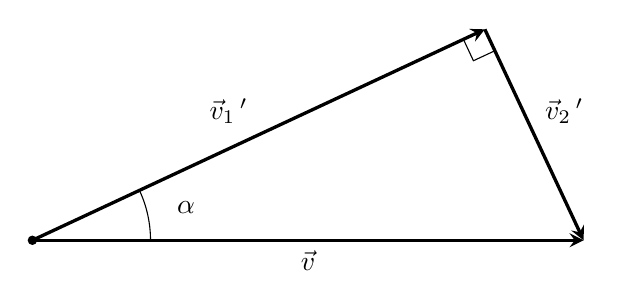
\begin{tikzpicture}[>=stealth]
 \draw[->, very thick] (0,0) -- (7,0) node[midway, below] {$\vec v$};
 \draw[->, very thick] (0,0) -- (5.746,2.679) node[midway, above left] {$\vec v_1\,'$};
 \draw[->, very thick] (5.746,2.679) -- (7,0) node[midway, above right] {$\vec v_2\,'$};
 \draw (1.5,0) arc (0:25:1.5);
 \node at (1.95,0.42) {$\alpha$};
 \draw (5.474,2.552) -- (5.601,2.28) -- (5.873,2.407);
 \fill (0,0) circle (0.06);
\end{tikzpicture}
\end{center}

Mit dem Ablenkwinkel $\alpha = \alBO$ des Spielballs ist
\begin{align}
 v_1' &= \vSnF = \vSp\cdot\cos\left(\alBO\right) = \vSn \approx \result{\vSnP{0}{2}} \\
 v_2' &= \vFaF = \vSp\cdot\sin\left(\alBO\right) = \vFa \approx \result{\vFaP{0}{2}}
\end{align}
Der Spielball rollt mit $v_1'$ weiter, die farbige Kugel mit $v_2'$, senkrecht zur Richtung des Spielballs.
